

\section{\tc Protocol}

We now describe the operation of \tc at the protocol level. The basic protocol is conceptually simple: A user contract \reqcont requests a datagram from the \tcontract \tcont. \tcont forwards the request to \engine and then returns the request to \reqcont. There are many details, however, relating to message contents and protection and the need to connect the off-chain parts of \tc with the blockchain.

First, we give a brief protocol overview. Then we enumerate the data flows in \tc. Finally, we provide a component-level view of the protocol by specifying the functionalities embodied in the \tcontract, \medname, and \encname. We present these  as ideal functionalities, inspired by the universal-composability (UC) framework, in order to abstract away implementation details and as a springboard for formal proofs of security. We omit details in this section on how payment is incorporated into \tc; this delicate aspect of the system design is deferred to Section~\ref{}.

\subsection{Datagram lifecycle}

The lifecycle of a datagram may be briefly summarized in the following steps:

\begin{itemize}
\item {\bf Initiate request.} \reqcont sends a datagram request to \tcont on the blockchain.

\item {\bf Monitor and relay.} The \medname monitors \tcont and relays any incoming datagram request with parameters \dgform to the \encname.

\item {\bf Securely fetch feed.} To process the request specified in \dgform, the \encname contacts a data source via HTTPS and obtains the requested datagram. It forwards the datagram via the Relay to \tcont.

\item {\bf Return datagram.} \tcont returns the datagram to \reqcont.
\end{itemize}

We now make this data flow more precise. 

\subsection{Data flows}

A datagram request by \reqcont takes the form of a message $m_1 = (\dgid, \dgcallback, \dgform)$ to \tcont on the blockchain. Here, $\dgid$ is a unique request identifier (which we explain later how to compute in practice); $\dgcallback$ specifies the entry point in \reqcont to which the datagram is to be returned. (In principle, $\dgcallback$ could specify an entry point in a different contract, but \tc does not yet adopt this generalization. $\dgform$ specifies the requested datagram, e.g., ${\sf params} := (\weburl, {\sf spec}, T)$, where $\weburl$ is the target data source and {\sf spec} specifies content of a the datagram to be retrieved (e.g., a stock ticker at a particular time), while $T$ specifies the delivery time for the datagram. 

\tcont forwards $m_2 = (\dgid, \dgform)$ to the \encname. It receives in return a return message $m_3 = (\dgid, \dgform, \dgm)$ from the $\tc$ service, where $\dgm$ is the datagram, i.e., contains the data (e.g., the desired stock ticker price). \tcont checks the consistency of $\dgform$ on the incoming and outgoing messages, and if they match forwards $\dgm$ to the entry point \dgcallback in \reqcont in message $m_4$. 

Fig.~\ref{fig:dataflow} shows the data flows involved in processing a datagram request. For simplicity, the figure omits the \medname, which is only responsible for data passing.


\begin{figure}[h!]
\centering
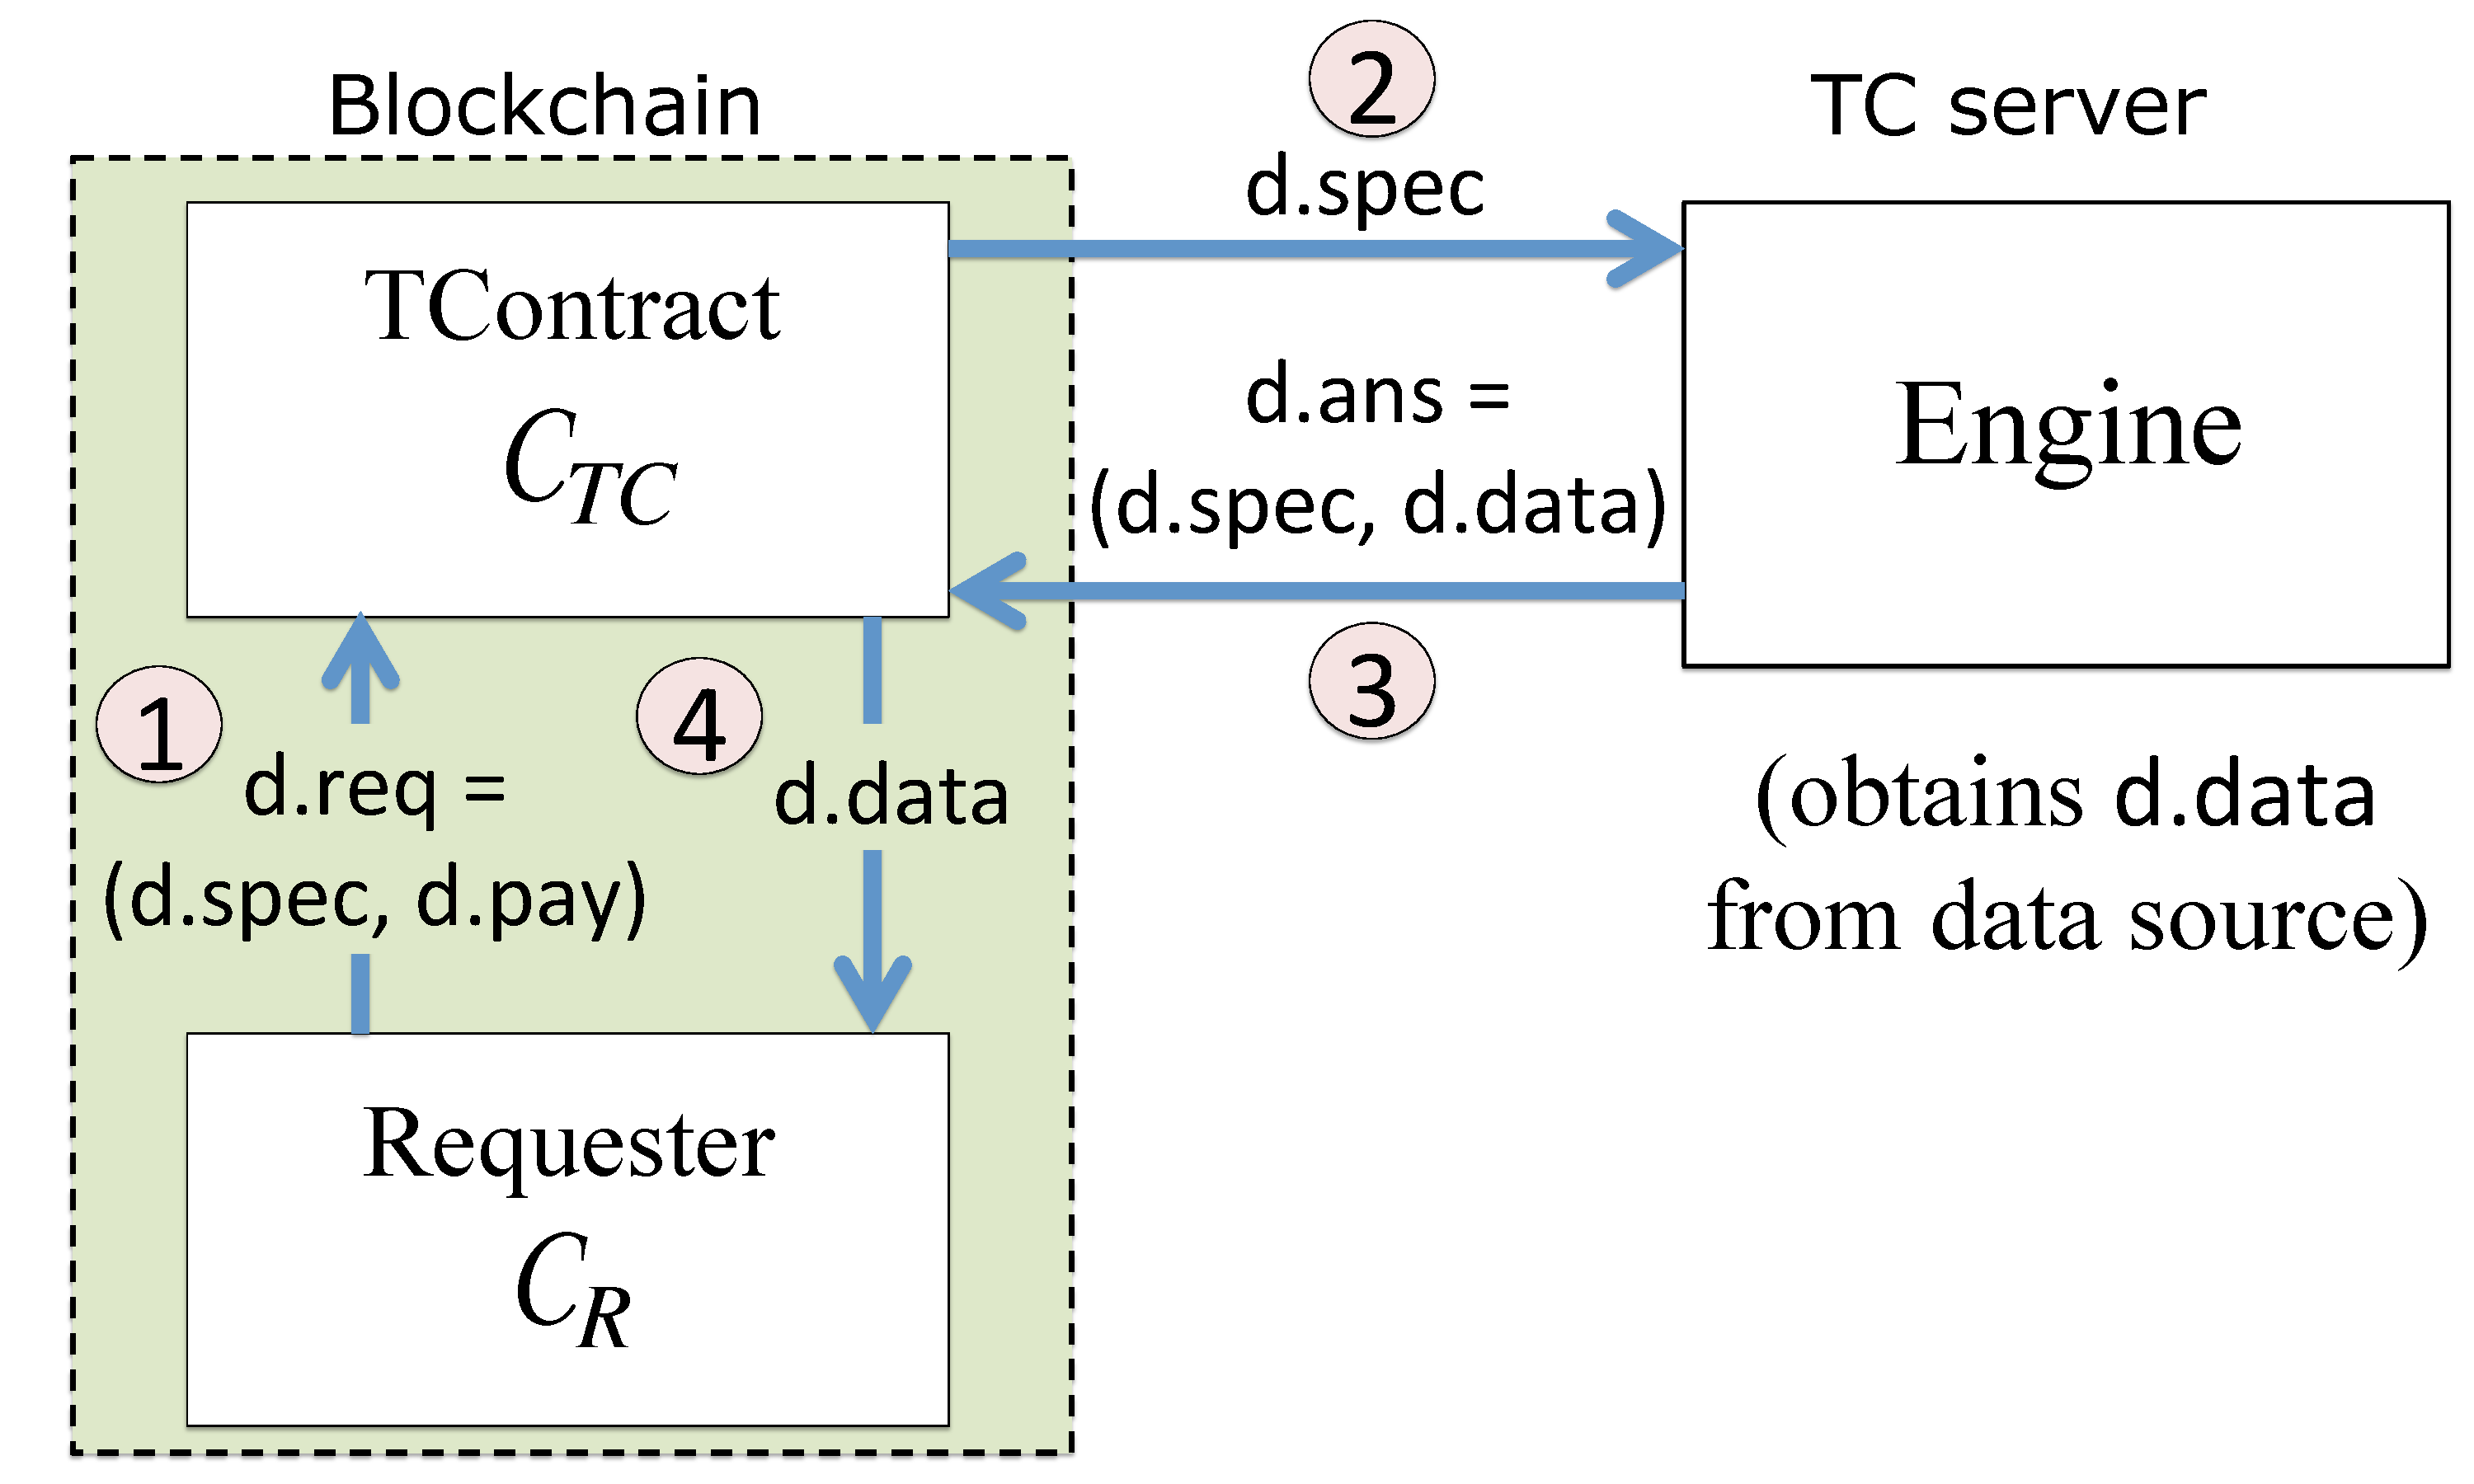
\includegraphics[width=\columnwidth]{figures/DataflowFig}
\caption{{\bf Data flows in datagram processing.}}
\label{fig:dataflow}
\end{figure}


Digital signatures are needed to authenticated messages, such as $\dgret$, entering the blockchain from an external source. We let $(\skTC, \pkTC)$ denote the private / public keypair associated with the \encname for such message authentication. For simplicity, Fig.~\ref{fig:dataflow} assumes that the Engine can send signed messages directly to \tcont. We explain shortly how Ethereum requires a slightly different approach in which \tc sends messages via an Ethereum wallet \tcadd.


\subsection{Use of SGX.}
Our protocols in \tc rely on the ability of SGX attestation to bind an instance of the \encname to a public key and for the \encname to maintain accurate absolute or wall-clock time. To simplify our presentation, we defer most details of our formal model of SGX capabilities and specification of protocols for attestation generation to the paper appendix. Instead, we first explain and present a simple abstraction of these capabilities suitable for our \tc protocol descriptions. 

Let $\enclaveprog$ represent the code for \encname, which we presume is trusted by all system participants. To avoid having to verify an EPID group signature on the blockchain, we have clients obtain SGX attestations from the \medname and verify them off-chain. As noted above, it is possible to bind an enclave process instance running \enclaveprog to a key pair $(\pkTC, \skTC)$ by including the public key pair in an attestation. We take this approach in \tc. 

\paragraph{Binding $\enclaveprog$ to Ethereum wallet \tcadd.}
Information can only be inserted into the blockchain in Ethereum as a transaction from a wallet. Thus, the only way the \medname can relay messages form the \encname to \tcont is through a wallet (again, formally, an externally owned account) \tcadd. Since the \medname may corrupt messages, however, it is critical that they be authenticated by the \encname. Since Ethereum itself 
already verifies signatures on transactions from externally owned accounts (i.e., users interact with the  Ethereum blockchain through an authenticated channel), \tc uses a trick to {\it piggyback verification of enclave signatures on top of Ethereum's already existing transaction signature verification mechanism}. 

Very simply, the \encname creates \tcadd with the public key \pkTC. 

To make this idea work fully, the public key $\pkTC$ must be hardcoded into \tcont. A client creating or relying on a contract that uses \tcont is responsible for making sure that this hardcoded $\pkTC$ has an appropriate SGX attestation before interacting with the $\tcont$  blockchain contract.  Let {\sf Verify} denote a verification algorithm for EPID signatures. Fig.~\ref{fig:att_check} gives the protocol for a client to check that \tcont is backed by a valid \encname instance. This protocol does not include a mechanism for \emph{revocation} of a compromised SGX instance, an issue we discuss later in the paper.

In summary, then, we may assume in our protocol specifications that {\em all relying clients have verified an attestation for \encname and thus that datagram responses passed from \tcadd to \tcont are trusted to originate from \engine.} 


\paragraph{\bf Clock.}
Additionally, as noted above, trusted clock provides only relative time with  respect to a reference point, not absolute time. Thus, when initialized, the \encname is provided with the current wall-clock time by a trusted source, e.g., the \medname (under a trust-on-first-use model). The SGX attestation generated by the \encname includes the current wall-clock time, which clients may verify in real time. Thus, a client can determine the absolute clock time of \encname to within a high degree of accuracy, bounded by the round-trip time of its attestation request plus the attestation verification time--on the order of hundreds of milliseconds in a wide-area network~\cite{}. A high degree of accuracy is potentially useful for some applications but sub-second accuracy is not required for most. Ethereum has a block interval of 12s and the clock serves in \tc primarily to: (1) Schedule connections to data sources and (2) To check TLS certificates for expiration when establishing HTTPS connections.
\ari{Let's give the attestation API a function name.} We present a formal model and protocol specification in the paper appendix.


\paragraph{\bf Notation.} We model execution in SGX in terms of a functionality $\fsgx$ operating in a stateful manner on \enclaveprog. This functionality may be be invokes through transmission of one of three messages to \enclaveprog: \initcall, which creates the enclave with \enclaveprog as its initial state and triggers measurement quotes, \attcall, which causes \engine to initiate an attestation with the public key and current time as supplementary data, and (\resumecall, $X$) which initiates an execution of \enclaveprog on a fresh input $X$. (We assume that \enclaveprog exits only when it completes processing of a given input.) We let $\fsgx[\enclaveprog, \relay]$ denote invocation of $\fsgx$ on \enclaveprog by \relay. We let $\clock()$ denote measurement of the SGX clock from within the enclave; $\clock()$ returns the current wall-clock time (in a canonical format such as seconds since the Unix epoch January 1, 1970 00:00 UTC).\ari{What format do we actually use?}

We abstract away the use of group signatures in EPID and simply denote the keypair associated with an SGX instance in \tc by $(\pkM, \skM)$. We let $\Sigma.{\sf Sign}({\sk}, X)$ denote a digital signature under private key $\sk$ of message $X$, and $\Sigma.{\sf Verify}({\sk}, \sigma, X)$ denote the corresponding verification operation.

\begin{figure}[htb!]
\begin{boxedminipage}{\columnwidth}
\begin{center}
{\bf User: offline attestation of SGX enclave}
\end{center}
\begin{tabular}{l}
{\bf Inputs}: $\pkM$, $\pkTC$, $\enclaveprog$, $\sigatt$ \\[5pt]
{\bf Checks:} \\
Assert $\enclaveprog$ is the expected enclave code\\
Assert $\sigsgx.{\sf Verify}(\pkM, \sigatt, (\enclaveprog, \pkTC))$ \\
Assert \tcont is correct and parametrized w/ \pkTC\\
{\it //~now okay to rely on \tcont}
\end{tabular}
\end{boxedminipage}
\caption{A client checks an SGX attestation on the enclave's code $\enclaveprog$ and public key $\pkTC$; the client
checks that $\pkTC$ is hardcoded into \tc blockchain contract \tcont before 
using \tcont.
} 
\label{fig:att_check}
\end{figure}


\begin{figure}
\begin{boxedminipage}{\columnwidth}
\begin{center}
{\bf $\fsgx[\enclaveprog, \relay]$: abstraction for SGX}
\end{center}
\begin{tabular}{l}
{\bf Hardcoded:} $\skM$ \\[5pt]

{\bf Assume:} \\ 
$\enclaveprog$ has entry points {\bf Initialize} and {\bf Resume}\\[5pt]

{\bf Initialize:}\\
On receive ``initialize'' from $\relay$: \\
\quad Let ${\sf outp} := \enclaveprog.{\bf Initalize}()$  \\
\quad $\sigatt := \sigsgx.{\sf Sign}(\skM, (\enclaveprog, {\sf outp}))$ \\[-1pt]
\qquad \qquad {\it //~models group sig.}\\
\quad Output  $({\sf outp}, \sigatt)$\\[5pt]

On receive (``resume'', ${\sf params}$) from $\relay$: \\
\quad Let ${\sf outp} := \enclaveprog.{\bf Resume}({\sf params})$  \\
\quad Output ${\sf outp}$ 
\end{tabular}
\end{boxedminipage}
\caption{Formal abstraction for SGX attested execution. 
We adopt a similar modeling approach by Shi et al., where
the SGX group signature is abstracted with a normal signature
by a manufacturer key $\pkM$. 
\elaine{cite our sok paper}
The above functionality only models a subset of SGX features
that is sufficient for our formalism.
}
\end{figure}


\paragraph{Formally abstracting SGX.}
\elaine{refer to figure and explain}



\subsection{A payment-free basic protocol}
For simplicity, we first specify functionalities in a payment-free version of our basic protocol, i.e., one that does not include gas or fees. Later, in our implementation discussion, we explain how we handle these two forms of payment, and we prove payment-related properties in the paper appendix. For simplicity, we assume a single instance of \engine and a since \tc server, although our architecture could scale up to multiple instances of either. To show messages corresponding to those in Fig.~\ref{fig:dataflow}, we use the label ({\bf msg.}~$m_i$)

\paragraph{The \tcontract \tcont.} The \tcontract, as noted above, accepts a datagram request $(\dgid, \dgform, \dgcallback)$, forwards it to the \tc server, and sends the resulting datagram $\dgm$ to the entry point \dgcallback in the requesting contract \reqcont. As we explain in Section~\ref{sec:implementation}, the blockchain verifies that the response is correctly signed under $\engine$'s key $\pkTC$, so \tcont need not verify the signature explicitly. \tc does, however, have a subtle security requirement. Specifically,  for a given datagram request $\dgid$, \tcont verifies that $\dgform' = \dgform$, where $\dgform$ is the digitally signed message produced by \engine and $\dgform$ is the locally stored parameters. The check is necessary to prevent \relay from corrupting datagram requests passed by \tcont (which, as a public function, has no means of digitally signing requests). \tcont is specified in Fig.~\ref{tbl:tc-contract}. As a reminder, we assume (and enforce) the condition that $\dgid$ is unique to a given request.

\begin{figure}[!htb]
\begin{tabularx}{\linewidth}{|@{\hspace{3pt}}r@{\hspace{1ex}}X@{\hspace{3pt}}|}
  \hline

  \multicolumn{2}{|c|}{{\bf Program for Town Crier blockchain contract \tcont}} \\ [1ex]
  {\bf Request:} & On recv $(\dgid, \dgform, \dgcallback)$ from some $\reqcont$:   
\\
& \qquad \qquad \qquad \qquad \qquad \qquad {\sgray{\it //~{\bf msg.}~$m_1$}} \\
%                 & If $(\${\sf fee} < F_{\rm min}$ or $\${\sf fee} > F_{\rm max})$ \\
%                 & \hspace*{1em} Return $\${\sf fee}$ to $\pkU$ \\
                 & Record $(\dgid, \dgform, \dgcallback)$ \\[5pt] 
%		 & Send $(\dgid, \dgform)$ to \relay \\
%\multicolumn{2}{|c|}{\sgray {\it // above implemented by \relay monitoring the blockchain}}\\[5pt]
  {\bf Deliver:} & On recv $(\dgid, \dgform, \dgm)$ from $\tcadd$: \\
		 & Let $(\dgid, \dgform', \dgcallback)$ be a most recently recorded tuple corresponding to $\dgid$ :\\
		 & Assert $\dgform = \dgform'$\\
                 & Call ${\dgcallback}({\dgm})$ \quad \sgray{\it //~{\bf msg.}~$m_4$}\\
%                 & Send $\${\sf fee}$ ether to $\Psgx$. \\

  \hline
\end{tabularx}
\caption{
The Town Crier \tcontract \tcont.
}
\label{tbl:tc-contract}
\end{figure}

\paragraph{The \encname \engine.} When initialized through an \initcall call, \engine sets its absolute clock (by setting a reference point) and generates a keypair $(\pkTC,\skTC)$ to which it binds by placing $\pkTC$ in attestation requests. Given input \resumecall $({\sf id}, {\sf params})$, \engine contacts the requested data source via HTTPS and checks that the corresponding certificate {\sf cert} is valid, i.e., not expired. We defer discussion of certificate revocation to Section~\ref{}. \engine then fetches the requested datagram and returns it to \relay along with the inputs, all digitally signed. The protocol for \engine is shown in Fig.~\ref{fig:engineprot}.

\begin{figure}[!h]
\begin{boxedminipage}{\columnwidth}
\begin{center}
{\bf Program for \tcs~\encname \engine (enclave)}
\end{center}
\begin{tabular}{l}
%{\bf Inputs}:  ${\sf params}$, \\[5pt]
%{\bf Initialize}:  On recv (\initcall, $T_0)$: \\ %{\it //~called only once upfront}\\
{\bf Initialize}:  On recv (\initcall): \\ %{\it //~called only once upfront}\\
%\quad Set clock reference point\\
%\quad Record $T_0$ \elaine{this is never used} \\ 
%\elaine{i deleted the clock implementation, we can separate abstraction from implementation.}\\
\quad $(\pkTC, \skTC) := \Sigma.{\sf KeyGen}(1^\lambda)$\\
%\quad Record $(\pkTC, \skTC)$\\
\quad Output $\pkTC$   \\
\sgray{\it/*$\fsgx$ attests to the code and the output $\pkTC$,} \\
\quad \sgray{see Figure \elaine{refer}*/}
\\[3pt]

%{\bf Attest}:  On recv \attcall: \\ %{\it //~called only once upfront}\\
%\quad $T := \clock()$\\
%\quad Call quoting enclave with supp.~data $(\pkTC, T)$
%\\[5pt]

{\bf Resume:} On recv (\resumecall, $({\sf id}, {\sf params}))$\\
\quad Parse ${\sf params} := (\weburl, \dgspec, T) $:\\
%\quad Parse ${\sf params} := (\weburl, \pkurl, T)$ \\
\quad Wait until $\clock() \geq T$\\
\quad Contact $\weburl$ via HTTPS, obtaining ${\sf cert}$ \\
\quad Verify {\sf cert} is valid for time $\clock()$\\
\quad Obtain webpage $w$ from $\weburl$ \\
\quad Parse $w$ to extract \dgm with specification (\dgspec, $T$) \\
\quad $\sigma := \Sigma.{\sf Sign}({\skTC}, ({\sf id}, {\sf params}, {\sf data}))$\\
\quad Output $(({\sf id}, {\sf params}, {\sf data}), \sigma)$
\end{tabular}
\end{boxedminipage}
\caption{
The \tcs~\encname \engine.
} 
\label{fig:engineprot}
\end{figure}

\paragraph{The \medname \relay.} As noted in Section~\ref{sec:architecture}, \relay performs distinct three forms of data passing, which we  specify more precisely here. It scrapes the blockchain, monitoring \tcont for new datagram requests $({\sf id}, {\sf params})$. It boots the \engine with an \initcall call and handles incoming requests by invoking \engine with \attcall or \resumecall calls. Finally, it forwards datagram responses from \engine to the blockchain; recall that it inserts data onto the blockchain and thus forward responses through \tcadd. The program for \relay is shown in Fig.~\ref{fig:relayprot}.

\begin{figure}[!h]
\begin{boxedminipage}{\columnwidth}
\begin{center}
{\bf Program for Town Crier \medname $\relay$}
\end{center}
\begin{tabular}{l}
{\bf Initialize}:\\
Send \initcall to $\fsgx[\enclaveprog, \relay]$\\
On recv $(\pkTC, \sigatt)$ from $\fsgx[\enclaveprog, \relay]$:\\
\quad Publish $(\pkTC, \sigatt)$\\[5pt]

{\bf  Loop forever}: \\
%{\bf Request}:
Whenever \tcont receives 
a request
$({\sf id}, {\sf params}, \_)$:  \\  %\sgray{{\it //~{\bf msg.}~$m_2$}}\\
%\quad Parse ${\sf params} := (\weburl, \dgspec, T)$\\
%\quad Fork: \\
\ \quad Send $(\text{\resumecall}, ({\sf id}, {\sf params}))$ to $\fsgx[\enclaveprog, \relay]$ \\
\ \quad On recv $(({\sf id}, {\sf params}, {\sf data}), \sigma)$ from $\fsgx[\enclaveprog, \relay]$:\\ 
\ \quad \quad  {\sf AuthSend} $({\sf id}, {\sf params}, {\sf data})$ to \tcont as \tcadd \\
\hspace{50mm}\sgray{\it //~{\bf msg.}~$m_3$}\\
\end{tabular}
\end{boxedminipage}
\caption{The Town Crier \medname \relay.}
\label{fig:relayprot}
\end{figure}



